% Part: sets-functions-relations
% Chapter: relations
% Section: trees

\documentclass[../../../include/open-logic-section]{subfiles}

\begin{document}

\olfileid{sfr}{rel}{tre}
\olsection{વૃક્ષો}

તર્કશાસ્ત્રના બધા ભાગોમાં મહત્વનો ભાગ ભજવતો આંશિક ક્રમનો
એક ખાસ પ્રકાર \emph{વૃક્ષ} છે. તર્કશાસ્ત્રના પ્રાથમિક ભાગોમાં
સાંત વૃક્ષો આવે છે: દાખલા તરીકે, !!{formula}sને વાક્યરચના
વૃક્ષમાં તેમના વિઘટન દ્વારા સમજી શકાય છે, જ્યારે ઘણી
!!{derivation} પદ્ધતિઓમાં !!{derivation}s પણ સાંત વૃક્ષોનું
રૂપ ધરાવે છે.
%
વિધાનાત્મક અને પ્રથમ ક્રમના તર્કશાસ્ત્ર માટેના પૂર્ણતા પ્રમેયોની
સાબિતીમાં જ અનંત વૃક્ષો દેખાય છે, અને ગાણિતિક તર્કશાસ્ત્રમાં
સર્વત્ર તેમનો ઉપયોગ થાય છે.

ગણસિદ્ધાંતમાં વૃક્ષનો ખ્યાલ, આલેખસિદ્ધાંતમાં વૃક્ષના ખ્યાલ સાથે
ગાઢ રીતે જોડાયેલો છે. અહીં એક (સાંત) વૃક્ષનું ચિત્ર છે:

\begin{center}
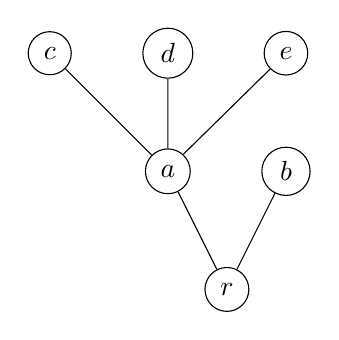
\begin{tikzpicture}[nodes={draw, circle}, -]
\node{$r$} [grow'=up]
    child { node {$a$}
        child { node {$c$} }
        child { node {$d$} }
        child { node {$e$} }
    }
    child { node {$b$} };
\end{tikzpicture}
\end{center}

સૌથી નીચેની ગાંઠ $r$ મૂળ છે. $r$ સિવાયની દરેક ગાંઠની
તરત નીચે બરાબર એક જનક ગાંઠ છે.
ગાંઠ $x$થી ધારોને અનુસરીને ઉપર જતાં ગાંઠ $y$ સુધી પહોંચી
શકાય ત્યારે $x$નો $y$ સાથેનો સંબંધ,
$x$ એ $y$નો \emph{પૂર્વજ} છે એમ સમજી શકાય.

વૃક્ષમાં પૂર્વજનો સંબંધ કડક આંશિક ક્રમ છે.
આ પરથી ગણસિદ્ધાંતની વ્યાખ્યા આપવાની પ્રેરણા મળે છે.
તે રજૂ કરવા માટે આપણને બે ખ્યાલો જોઈએ.
$\le$ વડે આંશિક ક્રમમાં ગોઠવેલા ગણ $A$માં
\emph{લઘુતમ ઘટક} એવો !!a{element} $x \in A$ છે
કે દરેક $y \in A$ માટે $x \le y$.
ગણ $\le$ વડે \emph{સુક્રમિત} હોય જો તેના દરેક
અરિક્ત ઉપગણમાં લઘુતમ ઘટક હોય.

\begin{defn}[વૃક્ષ]
\emph{વૃક્ષ} એવો જોડ $T = \tuple{A, \le}$ છે કે $A$ એક ગણ છે
અને $\le$ એ $A$ પરનો આંશિક ક્રમ છે, જેમાં એકમાત્ર લઘુતમ
ઘટક $r \in A$ છે (જેને \emph{મૂળ} કહે છે), અને
દરેક $x \in A$ માટે ગણ $\Setabs{y}{y \le x}$
એ $\le$ વડે સુક્રમિત છે.
\end{defn}

\begin{defn}[અનુગામીઓ]
ધારો કે $T = \tuple{A, \le}$ વૃક્ષ છે.
જો $x,y \in A$, $x < y$, અને $x < z < y$
થાય એવો કોઈ $z \in A$ ન હોય, તો આપણે કહીએ છીએ કે
$y$ એ $x$નો \emph{અનુગામી} છે.
\end{defn}

$x \in A$ના અનુગામીઓને તેની \emph{સંતાન ગાંઠો} પણ કહે છે.
જો $y$ એ $x$નો અનુગામી હોય, તો આપણે $x$ને $y$નો
\emph{પુરોગામી} અથવા \emph{જનક} કહીએ છીએ.

\begin{prop}
જો $\tuple{A,\le}$ વૃક્ષ હોય, તો મૂળ સિવાયના
દરેક $x \in A$નો વધુમાં વધુ એક પુરોગામી હોય.
\end{prop}

\begin{proof}
  ધારો કે $y_1 < x$ અને $y_2 < x$ અને $y_1 \neq y_2$.
  તો $\{y_1, y_2\} \subseteq \Setabs{z}{z<x}$.
  $\Setabs{z}{z<x}$ એ $\le$ વડે સુક્રમિત હોવાથી,
  તેના ઉપગણ $\{y_1, y_2\}$માં લઘુતમ ઘટક છે,
  જે દેખીતી રીતે કાં $y_1$ અથવા $y_2$ હોવો જોઈએ.
  તેથી કાં $y_1 \le y_2$ અથવા $y_2 \le y_1$.
  આપણે $y_1 \neq y_2$ ધાર્યું હતું, તેથી ખરેખર
  કાં $y_1 < y_2$ અથવા $y_2 < y_1$.
  આપણે $y_1 < x$ અને $y_2 < x$ ધાર્યું હોવાથી,
  વધુમાં કાં $y_1 < y_2 < x$ અથવા $y_2 < y_1 < x$.
  તેથી $y_1$ અને $y_2$ બંને $x$ના પુરોગામી હોઈ શકે નહીં.
\end{proof}

\begin{defn}
વૃક્ષ $T = \tuple{A, \le}$ \emph{અનંત} કહેવાય જો $A$
અનંત ગણ હોય, અને નહિતર \emph{સાંત} કહેવાય.
જો $T$માં દરેક $x \in A$ના માત્ર સાંત સંખ્યામાં અનુગામીઓ હોય,
તો આપણે કહીએ છીએ કે $T$ \emph{સાંત શાખનવાળું} છે.
\end{defn}

\begin{defn}[શાખાઓ]
વૃક્ષ $T = \tuple{A, \le}$ આપેલું હોય ત્યારે,
$T$ની \emph{શાખા} એ $T$માં સમાવેશની દૃષ્ટિએ મહત્તમ શૃંખલા છે,
એટલે કે, એવો ગણ $B \subseteq A$ કે કોઈ પણ
$x, y \in B$ માટે કાં $x \le y$ અથવા $y \le x$,
અને કોઈ પણ $z \in X \setminus B$ માટે એવો
$u \in B$ અસ્તિત્વ ધરાવે છે કે ન તો $z \le u$, ન તો $u \le z$.
%
આપણે $T$ની બધી શાખાઓના ગણને દર્શાવવા $[T]$ વાપરીએ છીએ.
\end{defn}

\begin{ex}
સાંત શાખનવાળા વૃક્ષનું એક સુપ્રસિદ્ધ ઉદાહરણ એ $0$ અને $1$ના
સાંત અનુક્રમોનું \emph{અનંત દ્વિઆધારી વૃક્ષ} છે,
જેને ક્યારેક $\{0,1\}^*$ અથવા $\Bin^*$થી દર્શાવવામાં આવે છે,
અને જે વિસ્તરણ સંબંધ $\sqsubseteq$ વડે ક્રમિત છે
(દા.ત., $101 \sqsubseteq 101101$).
કોઈ પણ દ્વિઆધારી પ્રતીકશ્રેણીને અંતે $0$ કે $1$ ઉમેરીને
હંમેશાં વિસ્તારી શકાય છે, તેથી આ વૃક્ષમાં અનંત સંખ્યામાં
ઘટકો છે: દરેક ઘટક $s$ના બરાબર બે અનુગામી $s0$ અને $s1$ છે.
તેનું મૂળ ખાલી અનુક્રમ $\emptyseq$ છે.
\end{ex}

\begin{ex}
થોડું વધુ સામાન્ય રીતે, વિસ્તરણ સંબંધ $\sqsubseteq$ સાથે
પ્રાકૃતિક સંખ્યાઓના સાંત અનુક્રમોનો ગણ $\Nat^*$ પણ વૃક્ષ છે.
તે દેખીતી રીતે સાંત શાખનવાળું નથી: દરેક $s \in \Nat^*$ના
અનંત સંખ્યામાં અનુગામી $sn$ છે, દરેક $n \in \Nat$ માટે એક.
$\sqsubseteq$ હેઠળ સંવૃત એવો દરેક $A \subseteq \Nat^*$
એ $\Nat^*$નું \emph{ઉપવૃક્ષ} છે.
(એટલે કે, $A$ એવો છે કે જો $s \in A$ અને
$s' \sqsubseteq s$, તો $s' \in A$ પણ.)
બધાં સાંત વૃક્ષોને $\Nat^*$નાં સાંત ઉપવૃક્ષો તરીકે રજૂ કરી શકાય છે.
\end{ex}

\begin{prop}[કેનિગનું સહાયક પ્રમેય]
જો $T = \tuple{A,\le}$ સાંત શાખનવાળું અનંત વૃક્ષ હોય,
તો $T$ને અનંત શાખા હોય છે.
\end{prop}

સંગણનીયતાના સિદ્ધાંતમાં વ્યાપકપણે વપરાતો કેનિગના સહાયક
પ્રમેયનો એક વિશેષ કિસ્સો, જેને \emph{નબળું કેનિગ સહાયક પ્રમેય}
કહે છે, આ છે: $\{0,1\}^*$ના કોઈ પણ અનંત ઉપવૃક્ષને
અનંત શાખા હોય છે.

\end{document}
